\section*{Unsupervised relationship mining}

% There are some limitations to modeling sentiment in a supervised way.
%   - Don't have explicit sentiment labels
%   - The interactions between countries is better described
%     by a dimension orthogonal to "war".
%     - Trade
%     - Culture and society

The preceding approach has limitations, however.  Sentiment labels
measure only one kind of interaction: whether countries are at war or
peace; but relationships between countries may be characterized in
many ways, some of which are independent of whether countries are at
war.  For example, the relationship between coutries may be
characterized by trade in goods, or by the exchange of culture and
society. Finally, these labels may be unavailable for a certain period
of time.

% in this section, we will describe a model which will allow us to discover
% unsupervised relationships
%   - We will use a modul much like RTM
%   - RTM is ...
In this section we will describe a model for inferring relationships
between countries in an unsupervised fashion.  This model serves as an
alternative to the model in the last section in that it requires no
explicit labels of the relationship between two different countries.
Instead, it infers a qualitative relationship between countries which
we will interpreted post-hoc.

The significance of this approach is that it infers a relationship
between countries based more on the discussion of these countries than
explicit labels.  This will allow us to qualify the discussion of
foreign relations.

We will begin by outlining a language model for this purpose.  We will
outline the key assumptions of this model -- namely, that a an
exposition about two countries comprises language about each country,
language about their relationship, and language from some background
distribution. We then describe inference for this model, and finally
provide an empirical analysis using this model.

\subsection{A model of unsupervised relationship.}
% The assumptions are as follows:
%   - Each country is associated with a background distribution
%   - Each interaction is described by:
%     - words related to either country
%     - miscellaneous words
%     - words about the relationship between the two countries
In the supervised foreign relations discourse model, our aim is to
characterize the relationship between two countries by inspecting the
language used to describe them.  This model comprises two pieces: a
language model for describing the language used to discuss countries;
and a time-series spatial model to describe the relationship between
pairs of countries.  We will begin by outlining the spatial sentiment
model, which will be familiar to readers from the last section.  We
then describe the language model, which is similar to LDA.  We then
describe how these two models are connected.

\subsubsection*{Dynamic spatial model}
The assumptions for interaction between countries in the unsupervised
model are similar to those we used in the supervised model from the
last section.  Each country is characterized by a position $\bar
x_{ct}$ which drifts over time in some latent space $\mathbb{R^d}$.
Pairs of countries interact according to the dyadic relationship
\begin{align}
  x_{c_1,d} | \bar x_{c_1,t} & \sim \mathcal{N}(\bar x_{c_1, t}, \sigma_s^2) \nonumber \\
  x_{c_2,d} | \bar x_{c_2,t} & \sim \mathcal{N}(\bar x_{c_2, t}, \sigma_s^2) \nonumber \\
  s_d | x_{c_1,d}, x_{c_2,d}, r_{c_1,d}, r_{c_2,d} & = \log( || x_{c_1,d} - x_{c_2,d} ||_2^2 + 1), \nonumber \\
  \kappa_d | s_d & \sim \sigma(s_d),
\end{align}
where each country $c$ has an additional intercept $r_c$ and
$\sigma(s)$ is the logistic function $\frac{\exp(s)}{1 + \exp(s)}$.
We illustrate this graphically in \myfig{dyadic_chain}.  As in the
last section, we use the extra variables $x$ instead of $\bar x$ for
computational convenience because we can estimate $\bar x$ over time
using a Kalman filter.

Also as before, we attach an intercept $\bar r_{c_2}$ to each country
to model each country's typical interaction style.  This gives us the augmented model
\begin{align}
  r_{c_1,d} | \bar r_{c_1} & \sim \mathcal{N}(\bar r_{c_1}, \sigma_r^2) \nonumber \\
  r_{c_2,d} | \bar r_{c_2} & \sim \mathcal{N}(\bar r_{c_2}, \sigma_r^2) \nonumber \\
  s_d | x_{c_1,d}, x_{c_2,d}, r_{c_1,d}, r_{c_2,d} & = \log( || x_{c_1,d} - x_{c_2,d} ||_2^2 + 1)  + r_{c_1} + r_{c_2} \nonumber \\
  \kappa_d | s_d & \sim \sigma(s_d)
\end{align}
We illustrate this sentiment model graphically in \myfig{dynamic_dyadic_chain}.

The sentiment parameter $\kappa_d$ will become important when we link
this sentiment model to text.  Intuitively, if two countries in
document are far apart in the latent space, we expect that $\kappa$ is
more likely to be 1.  Otherwise, $\kappa$ is more likely to be 0.  As
we develop the language model, we will use this random variable to
select a topic used to describe pairs of countries.

\subsubsection*{Binary Relational language model}
We incorporate text using a mixed-membership language model similar to
LDA.  Recall that in LDA, each word comes from a specific topic.  In
our model, which we dub the \emph{binary relational language model},
we assume that the words describing a pair of countries come from
topics about those countries.

\paragraph{A mixture of four topics.} To be concrete, consider a document discussing Iran and the United
States.  Each word in this document will serve one of
four roles:
\begin{enumerate}
  \item It discusses the U.S. only,
  \item It discusses Iran only,
  \item It discusses the relationship between the U.S. and Iran. \label{foreign_relations:relationship}
  \item It is a ``filler'' word, providing little contribution to the discussion. \label{foreign_relations:filler}
\end{enumerate}
The first two roles are self-explanatory.  The relationship in
(\ref{foreign_relations:relationship}) above could be any type of
relationship -- the goal of this section is of course to discover the
relationships in a collection of documents about these
countries.  The ``filler'' words in
(\ref{foreign_relations:filler}) above are those words found in any document
-- stopwords, for example -- that are unrelated to either country or
the relationship between them.

We therefore keep $(N_c + 2 + 1)$ topics---topics $\beta_{C,1},
\ldots, \beta_{C,{N_c}}$ for each of the $N_c$ countries, exactly two
sentiment topics $\beta_{S,0}, \beta_{S,1}$, and a single, global
background topic $\beta_{B0}$ \cite{chemudugunta:2009}.  We assume, as in LDA, that a document
about the United States and Iran is a mixture of topics; in contrast
to LDA, we constrain this document's topics to be exactly the four
topics enumerated above: $\beta_{C,\mbox{\tiny Iran}}$,
$\beta_{C,\mbox{\tiny United States}}$, $\beta_{B,0}$, and either
$\beta_{S,0}$ or $\beta_{S,1}$ (we describe below how to make the
choice between $\beta_{S,0}$ and $\beta_{S,1}$).  A document about
Hungary and Germany, in contrast, would be a mixture of the topics
$\beta_{C,\mbox{\tiny Germany}}$, $\beta_{C,\mbox{\tiny Hungary}}$,
$\beta_{B,0}$, and either $\beta_{S,0}$ or $\beta_{S,1}$.

Once these topics are fixed for a document, the language model
proceeds exactly as with LDA: each word in the document comes from one
of four topics, with probability for topic $k$ proportional to the
document-topic mixture weights $\theta_{dk}$.  We illustrate this
model graphically in \myfig{binary_relational_language_model}.

\subsubsection{Determining the sentiment topic: connecting dyadic sentiment and text}

Up to now the dyadic sentiment model and the language model have been
developed independently.  We connect the two models by using the binary
sentiment parameter $\kappa_d$ to index the sentiment topic for a
document: document $d$ takes topic $\beta_{S,\kappa_d}$ for its
sentiment topic.\footnote{We also make a small adjustment to ensure
  that the model converges to a reasonable mode.  There are two main
  components of this model: a language model and a sentiment model. We
  introduce a parameter $\nu \sim \mathbb{N(0, 100)}$ and per-document
  parameters $\nu_d \sim \mathbb{R}(\nu, 0.001)$ and define the binary
  sentiment $\kappa_d \sim \sigma(s_d \nu_d)$.}
% determine the sentiment topic based on $k$.
In other words, if two countries are far apart in the latent space,
then when they interact in document $d$, this interaction is likely to
be negative (i.e., $\kappa_d = 1$, and the language used to
describe their relationship will come from topic $\beta_{S, 1}$.  If
they were instead close together in this latent space, the language used to describe their relationship would come from topic $\beta_{S, 0}$.


We can now specify the generative model of a document language, given
the sentiment $\kappa_d$ for each interaction between countries.  We
begin by specifying the global topics.
\begin{enumerate}
\item First, draw topics:
  \begin{enumerate}
  \item For nation $c=1, \ldots, C$:
    \begin{itemize}
    \item Draw topic $\beta_{\mbox{C},c} \sim \mbox{Dir}(1, \ldots, 1)$.
    \end{itemize}
  \item Draw background topic $\beta_{\mbox{B},0} \sim \mbox{Dir}(1, \ldots, 1)$.
  \item Draw positive-interaction topic $\beta_{\mbox{S},0} \sim \mbox{Dir}(1, \ldots, 1)$
  \item Draw negative-interaction topic $\beta_{\mbox{S},1} \sim \mbox{Dir}(1, \ldots, 1)$
\end{enumerate}

\item Next, draw documents. \\
For document $d=1, \ldots, D$, each representing interactions between pairs of countries $c_{d_1},c_{d_2}$:
  \begin{enumerate}
    \item Draw topic mixture $\theta_d \sim \mbox{Dir}(1, 1, 1, 1)$
    \item Draw sentiment index $\kappa_d \sim \sigma(s_d)$
    \item For word $n = 1, \ldots, N_d$:
    \begin{itemize}
      \item Draw $z_{n} \sim \mbox{Mult}(\theta_d$).
      \item Switch($z_n$):
      \begin{itemize}
        \item If $z_n = (1, 0, 0, 0)$, draw $w_n \sim \beta_{\mbox{C},c_{d_1}}$.
        \item If $z_n = (0, 1, 0, 0)$, draw $w_n \sim \beta_{\mbox{C},c_{d_2}}$.
        \item If $z_n = (0, 0, 1, 0)$, draw $w_n \sim \beta_{\mbox{B},0}$.
        \item If $z_n = (0, 0, 0, 1)$, draw $w_n \sim \beta_{\mbox{S},\kappa_d}$.
      \end{itemize}
    \end{itemize}
  \end{enumerate}
\end{enumerate}
We illustrate the combined model in
\myfig{dynamic_dyadic_chain_binary_relational_language_model}.

\subsubsection{Related work: relational topic models}
The binary relational language model is founded on ideas discussed by
several recent models.  Chang et al. developed a model to describe the
relationships between entities with a similar assumption of
entity-specific and relationship-specific topics
\cite{chang:2009nubbi}.  In their \emph{Networks Uncovered by Bayesian
  Inference} (Nubbi) model, topics described the ``context''
surrounding either entities (countries) or relationships (interactions
between countries).  The goal of Nubbi was to infer relationships
between entities.

The idea of a background topic was researched by
Chemudugunta et al. \cite{chemudugunta:2009}.

Neither of these sources included a switch variable for interaction topics.

\begin{figure}
  \center
  \begin{tabular}{lm{2.5in}lm{2.5in}}
    \begin{tabular}{c}
      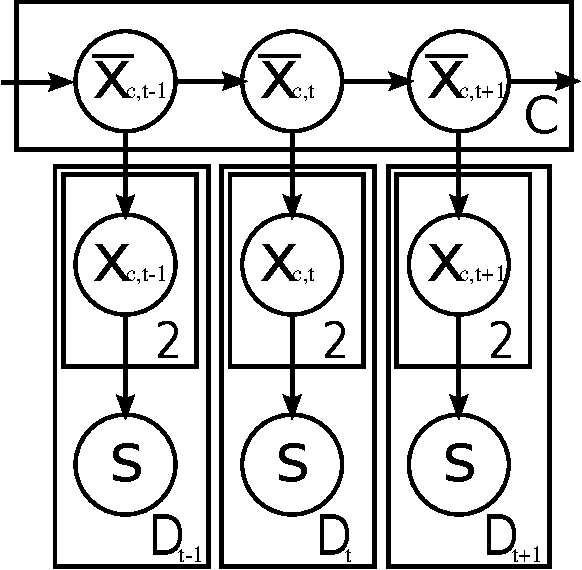
\includegraphics[width=0.26\textwidth]{chapter_foreign_relations/figures/countries_gm_no_text.pdf} \\ (A) \vspace{50pt} \\
      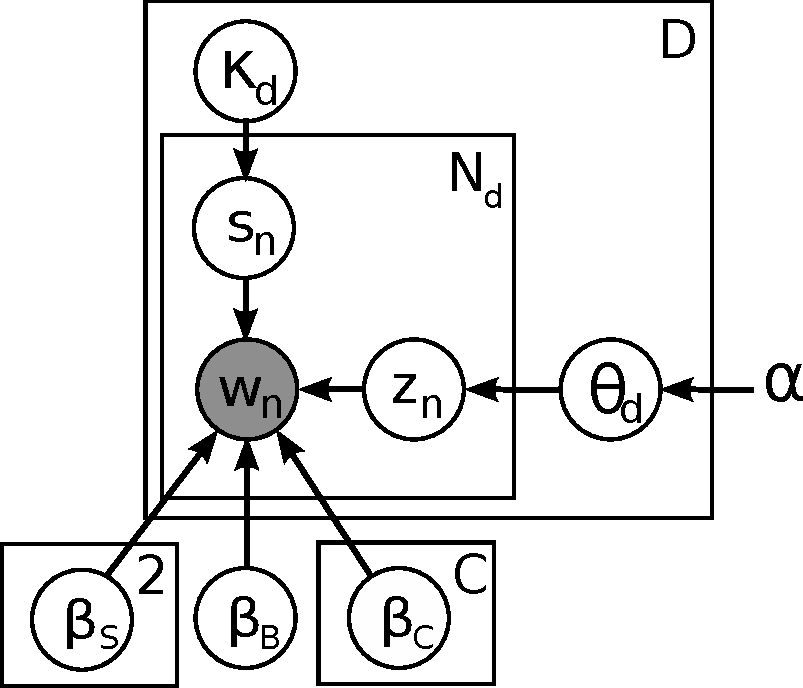
\includegraphics[width=0.35\textwidth]{chapter_foreign_relations/figures/fr_lda_gm.pdf} \\ (B) \\
    \end{tabular}
    &
    \begin{tabular}{c}
    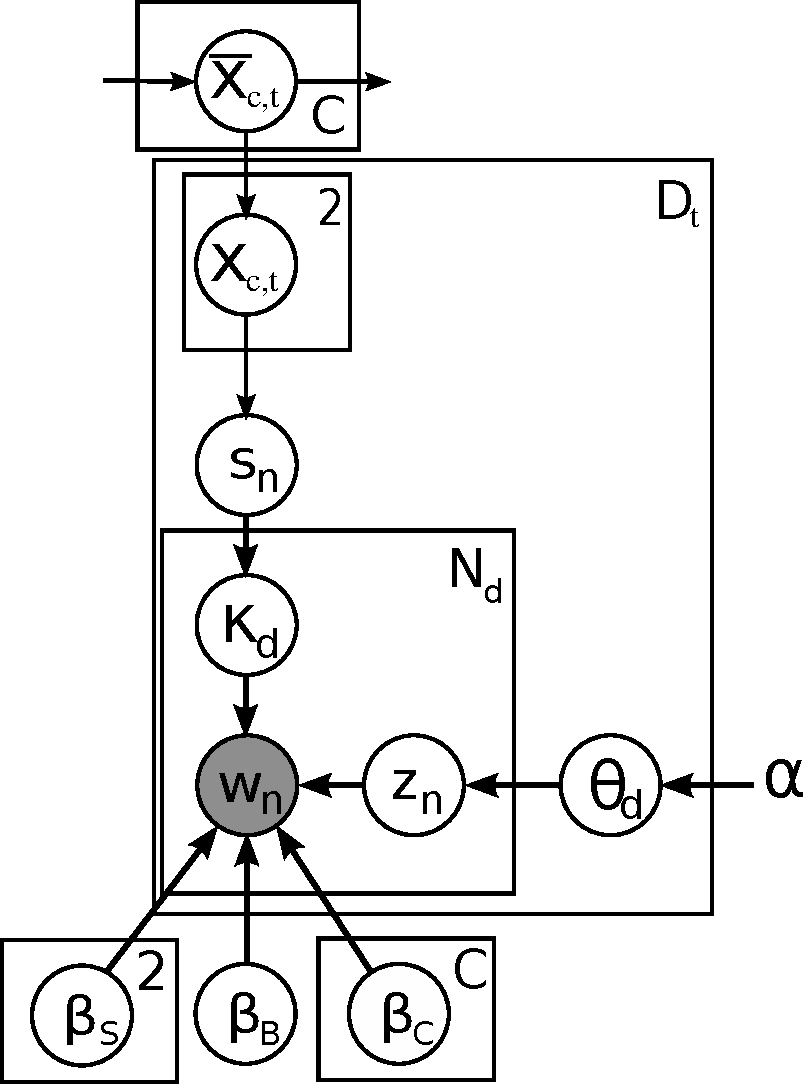
\includegraphics[width=0.35\textwidth]{chapter_foreign_relations/figures/countries_gm_unsupervised_all.pdf} \\ (C) \\
    \end{tabular}
  \end{tabular}
  \caption{The dynamic sentiment model (A), a binary mask
    mixed-membership language model (B), and the full unsupervised
    foreign relations model (C) (which is a combination of (A) and
    (C).  In (B) and (C), we assign each country its own topic
    $\beta_{C,\cdot}$.  Interactions between countries are
    characterized by sentiment $s_d$, which is reflected in the
    sentiment topic $\beta_{S,\kappa_d}$.  The background topic
    $\beta_B$ is provided to ``soak up'' background noise.}
  \label{fig:dynamic_dyadic_chain}
  \label{fig:binary_relational_language_model}
  \label{fig:dynamic_dyadic_chain_binary_relational_language_model}
\end{figure}

\subsection*{Empirical analysis}

\subsubsection*{Quantitative evaluation}
\paragraph{Perplexity}
% comparison with LDA, for a variety of topics.
% comparison with 
\paragraph{Sentiment}

\paragraph{Relationship between sentiment and third-party sentiment}

\subsubsection*{Topics}

\paragraph{An economics/military dichotomy.}
The sentiment topic is particularly telling.  Again using the
convention that $\kappa_d=1$ indicates \emph{negative} sentiment
between countries, the negative-sentiment topic $\beta_{S,1}$ matches
our intuition: it contains words typically associated with the
sentiment between warring states:

% What do the topics look like?
%  background topic?

\begin{table}
%         Country
% 2   united_states
% 3            iran
% 4           japan
% 8          canada
% 13          china
% 17           iraq
% 24        ireland
% 31  great_britain
% 243            X1
%                                                                                             Topics
% 2   officials,military,official,policy,political,support,government,meeting,leaders,administration
% 3                             nuclear,war,program,weapons,officials,arms,oil,hostages,gulf,uranium
% 4               trade,economic,countries,officials,market,economy,world,military,companies,markets
% 8                      trade,country,free,province,border,agreement,speaking,percent,law,officials
% 13               rights,human,trade,relations,officials,nuclear,visit,political,democracy,economic
% 17               forces,weapons,military,troops,officials,government,security,war,chemical,country
% 24                     police,people,province,peace,killed,political,bomb,control,violence,killing
% 31          officials,government,authorities,intelligence,week,people,minister,colony,time,country
% 243             war,political,officials,country,people,military,international,peace,confirmed,week
% mexico: drug,officials,border,law,enforcement,traffickers,agents,police,authorities,trade,cocaine,illegal
  \center
\begin{tabular}{|c|c|}
  \hline
  \textbf{Background topic ($\beta_{B}$)} \\
  \hline
  war \\
  political \\
  officials \\
  country \\
  people \\
  military \\
  international \\
  peace \\
  confirmed \\
  week \\
  following \\
  government \\
  \hline
\end{tabular}
\hspace{30pt} \begin{tabular}{|cc|}
  \hline
  \textbf{Economics topic ($\beta_{S,0}$) vs.} &
  \textbf{Military topic ($\beta_{S,1}$)} \\
  \hline
  million & military \\
  percent & officials \\
  people & soldiers \\
  billion & killed \\
  oil & troops \\
  officials & police \\
  country & forces \\
  money & people \\
  aid & attack \\
  government & border \\
  companies & near \\
  military & air \\
  \hline
\end{tabular}
\\
\vspace{30pt}
\begin{tabular}{|c|c|c|}
  \hline
  \textbf{Pakistan ($\beta_{C,\mbox{\tiny Pakistan}}$)} &
  \textbf{Mexico ($\beta_{C,\mbox{\tiny Mexico}}$)} &
  \textbf{Israel ($\beta_{C,\mbox{\tiny Israel}}$)} \\
% Iran: nuclear,war,program,weapons,officials,arms,oil,hostages,gulf,uranium
% China: rights,human,trade,relations,officials,nuclear,visit,political,democracy,economic
% india: nuclear,countries,border,weapons,tests,talks,nations,military,state,territory,war,militants
% pakistan: nuclear,weapons,military,officials,terrorism,border,war,government,aid,support,countries,militants
% mexico: drug,officials,border,law,enforcement,traffickers,agents,police,authorities,trade,cocaine,illegal
% israel: peace,territories,occupied,talks,officials,negotiations,agreement,state,settlement,security,settlements,violence
  \hline
  nuclear & drug & peace \\
  weapons & officials & territories \\
  military & border & occupied \\
  officials & law & talks \\
  terrorism & enforcement & officials \\
  border & traffickers & negotiations \\
  war & agents & agreement \\
  government & police & state\\
  aid & authorities & settlement \\
  support & trade & security \\
  \hline
\end{tabular}
\vspace{10pt}
\begin{tabular}{|c|c|c|}
  \hline
  \textbf{United States ($\beta_{C,\mbox{\tiny United States}}$)} &
  \textbf{Iran ($\beta_{C,\mbox{\tiny Iran}}$)} &
  \textbf{China ($\beta_{C,\mbox{\tiny China}}$)} \\
% Iran: nuclear,war,program,weapons,officials,arms,oil,hostages,gulf,uranium
% China: rights,human,trade,relations,officials,nuclear,visit,political,democracy,economic
% india: nuclear,countries,border,weapons,tests,talks,nations,military,state,territory,war,militants
% pakistan: nuclear,weapons,military,officials,terrorism,border,war,government,aid,support,countries,militants
% mexico: drug,officials,border,law,enforcement,traffickers,agents,police,authorities,trade,cocaine,illegal
  \hline
  officials & nuclear & rights \\
  military & war & human \\
  official & program & trade \\
  policy & weapons & relations \\
  political & officials & officials \\
  support & arms & nuclear \\
  government & oil & visit \\
  meeting & hostages & political \\
  leaders & gulf & democracy \\
  administration & uranium & economic \\
  \hline
\end{tabular}
\caption{Per-country topics ($\beta_{C,\cdot}$), a background topics ($\beta_{B,0}$), and the two interaction topics ($\beta_{S,0}, \beta_{S,1}$).}
\label{table:fr_unsupervised_topics}
\end{table}
\paragraph{National topics}



